\documentclass[twocolumn]{aastex701}
\usepackage{amsmath}

\newcommand{\kext}{\kappa_{\rm ext}}
\newcommand{\dmu}{\Delta\mu}
\newcommand{\msun}{M_\odot}
\newcommand{\snk}{\texttt{SNKappa}}

\shorttitle{Predicted lensing magnification of DES supernovae}
\shortauthors{Nugent et al.}

\begin{document}

\title{Weak Lensing Magnification of Type Ia Supernovae in the Dark Energy
Survey Five-Year Sample from a Predicted External-Convergence Model}

\author[0000-0002-3389-0586]{Peter E. Nugent}
\affiliation{Lawrence Berkeley National Laboratory, 1 Cyclotron Road,
Berkeley, CA 94720, USA}
\affiliation{Department of Astronomy, University of California, Berkeley,
CA 94720-3411, USA}
\email{penugent@lbl.gov}
%% co-authors TBD

\begin{abstract}
We present a detection of weak gravitational lensing magnification of
Type~Ia supernovae (SNe~Ia) in which the lensing signal is
\emph{predicted}, rather than fitted, from the foreground galaxy and
cluster distribution. Using only public data --- DESI Legacy Imaging
Surveys DR10 photometry and photometric redshifts, DESI DR1 spectroscopy,
and the Wen \& Han cluster catalog --- we compute the external convergence
$\kext$ along the sight line to each of 1450 high-probability SNe~Ia in
the Dark Energy Survey five-year sample (DES-SN5YR), assigning each
foreground galaxy a dark-matter halo through an independently calibrated
stellar-mass--halo-mass chain and injecting clusters as single halos with
miscentering and richness-scatter marginalization. Correlating the
predicted $\kext$ with the published DES Hubble residuals yields a slope
$d\dmu/d\kext = -2.10 \pm 0.47$~mag, in agreement with the theoretical
expectation of $-5/\ln 10 = -2.17$ for weak lensing: the ratio of observed
to predicted lensing amplitude is $A = 0.96 \pm 0.22$, a $4.4\sigma$
detection confirmed non-parametrically (Spearman $p = 1\times10^{-4}$).
The 202 sight lines with $\kext > 0.005$ are on average
$0.033 \pm 0.012$~mag brighter than the remainder. Because the amplitude
is predicted, the measurement simultaneously detects lensing and validates
the adopted galaxy--halo connection at the population level,
complementing the residual-fitted detection of Shah et al. We release the
per-supernova $\kext$ catalog, which enables environmental de-lensing and
the identification of individual magnification outliers in cosmological
samples.
\end{abstract}

\keywords{Gravitational lensing (670) --- Type Ia supernovae (1728) ---
Cosmology (343)}

\section{Introduction}\label{sec:intro}

Weak gravitational lensing by foreground large-scale structure perturbs
the observed brightnesses of Type~Ia supernovae (SNe~Ia), introducing a
redshift-dependent, skewed scatter into the Hubble diagram with
$\sigma_{\rm lens} \simeq 0.055z$~mag \citep{Holz2005,Jonsson2010}. In
current cosmological analyses this effect is treated statistically, as a
Gaussian contribution to the distance-modulus uncertainty; the DES
five-year analysis \citep[DES-SN5YR;][]{Abbott2024} notes explicitly that
the non-Gaussian tail imprinted by lensing magnification is otherwise
uncorrected, and the released Hubble-diagram lensing correction column is
identically zero.

The information discarded by the statistical treatment is recoverable:
the same foreground galaxies that source the convergence are catalogued
by wide-field surveys. \citet{Shah2022} searched for the corresponding
correlation in the Pantheon sample with marginal significance, and
\citet{Shah2024} achieved the first $>5\sigma$ detection by correlating
DES-SN5YR Hubble residuals with DES Y3 foreground galaxies, modeling
each galaxy as a halo whose mass-to-light normalization and profile were
\emph{fitted to the residuals themselves}. That design measures the
correlation optimally but cannot test the expected amplitude: the fitted
normalization absorbs any error in the assumed galaxy--halo connection.

In this Letter we take the complementary approach: the per--sight-line
convergence is predicted with no reference to the Hubble residuals, using
a halo model calibrated entirely on external data. The prediction machinery
(\snk) was developed for the environment analysis of the strongly lensed
SN 2025wny \citep[][M\"ortsell et al. 2026, in preparation]{Goobar2026}
and validated there against deep-SED stellar masses and null tests, as
well as against the classical line-of-sight magnification case of
SN~1997ff \citep{Benitez2002}. Applied to DES-SN5YR, it converts the
lensing detection into a measurement of the ratio of observed to predicted
lensing amplitude --- a population-level test of the galaxy--halo
connection using supernova magnification, analogous in spirit to
galaxy--galaxy lensing but with standard candles as the sources.

\section{Data}\label{sec:data}

\emph{Supernovae.} We use the public DES-SN5YR Hubble diagram and
metadata \citep{Abbott2024,Sanchez2024,Vincenzi2024}: distance moduli
$\mu$, uncertainties, BEAMS Type-Ia probabilities $P_{\rm Ia}$, host
coordinates, and field assignments. We select the 1572 SNe in the ten DES
fields with $0.1 < z_{\rm HD} < 1.15$ and valid host positions, adopting
the host coordinates as the sight line (host--SN offsets are negligible at
the arcminute scales relevant here); the 194 external low-redshift SNe
are excluded ($\sigma_{\rm lens} < 5$~mmag). Our baseline sample applies
$P_{\rm Ia} > 0.9$ (1450 SNe). Hubble residuals $\dmu$ are computed
against flat $\Lambda$CDM with $\Omega_{\rm M}=0.352$ \citep{Abbott2024}
with the weighted mean subtracted; no other transformation is applied to
the published distances.

\emph{Foregrounds.} For each of the four field groups (XMM-LSS, Stripe
82, CDF-S, Elais-S1) we build one regional catalog from the DESI Legacy
Imaging Surveys DR10 \citep{Dey2019}: \texttt{Tractor} sources with
standard quality cuts, Milky Way--dereddened $griz$+WISE fluxes, and a
depth limit of $z \le 22.5$~mag, yielding $(1.3$--$5.6)\times10^5$
galaxies per region. Photometric redshifts are the DR10 random-forest
estimates \citep{Zhou2021}, with $p(z)$ reconstructed from the released
quantiles; DESI DR1 spectroscopic redshifts \citep{DESI2025} supersede
them where available ($1.9\times10^4$ and $1.4\times10^4$ galaxies in the
XMM-LSS and Stripe~82 regions; the southern CDF-S and Elais-S1 fields lie
outside the DESI footprint). Galaxy clusters are taken from
\citet{WenHan2024}, 1600--1900 per region.

\section{Method}\label{sec:method}

Each foreground galaxy is assigned a halo as follows. Stellar masses come
from the rest-frame 1\,$\mu$m luminosity, obtained by log-interpolating
each galaxy's own $z$-band and WISE W1 fluxes to the observed wavelength
$(1+z)\,\mu$m --- a per-galaxy, data-driven K-correction --- with
$M_\star/L_{1\mu m} = 0.6$ \citep{Meidt2014,Kettlety2018}. Halo masses
follow by inverting the stellar-to-halo-mass relation of
\citet{Behroozi2013}, capped at $M_{200c} = 10^{13.8}\,\msun$ for
individual galaxies; concentrations use \citet{DiemerJoyce2019}; and each
halo is a truncated NFW profile \citep{BMO2009} with truncation at
$r_{200c}$. The convergence contributed by galaxy $i$ at angular
separation $\theta_i$ from a sight line to a source at $z_s$ is
\begin{equation}
\kappa_i = \frac{\Sigma_i\!\left(\theta_i D_A(z_i)\right)}
{\Sigma_{\rm cr}(z_i, z_s)},
\end{equation}
evaluated at the spectroscopic redshift where available and marginalized
over $p(z)$ otherwise. Clusters are injected as single NFW halos
($M_{200} = 1.4\,M_{500}$, $c=5$) with their member galaxies' halos
removed (replacement, not addition), and their contribution is
marginalized over a Rayleigh miscentering of $30''$ and a 0.25~dex
richness--mass scatter. The mass-sheet zero point is defined empirically:
the identical estimator is evaluated on 120 random sight lines per field
per source-redshift bin, and
\begin{equation}
\kext = \Big[\textstyle\sum_i \kappa_i + \kappa_{\rm cl}\Big]_{\rm SN}
- \Big\langle\textstyle\sum_i \kappa_i + \kappa_{\rm cl}\Big\rangle_{\rm rand}.
\end{equation}
Source redshifts are binned with $\Delta z_s = 0.05$. In the weak-lensing
limit the induced distance-modulus shift is $\dmu = -(5/\ln 10)\,\kext =
-2.171\,\kext$~mag, which is the prediction tested below; no parameter of
the model is adjusted against the Hubble residuals.

The mass scale carries four independent validations from the companion
work: (i) the estimator reproduces the deep-SED Prospector mass of the
SN 2025wny primary lens to 0.04~dex; (ii) a 487-galaxy calibration
campaign against the FrankenBlast SBI++ SED-inference engine
\citep{Nugent2025} measures the estimator scatter adopted here
(0.16~dex); (iii) a blank-field null test returns
$\kext = -0.008 \pm 0.010$; and (iv) applied to the SN~1997ff sight line
with HDF-quality inputs, the model reproduces the Keck-kinematics lower
limit on that supernova's magnification \citep{Benitez2002}. The full
DES computation --- four regional catalogs, $\sim$12{,}000 sight-line
evaluations --- takes 26 minutes on a desktop; all queries, versions, and
seeds are recorded for exact reproduction.

\begin{figure}
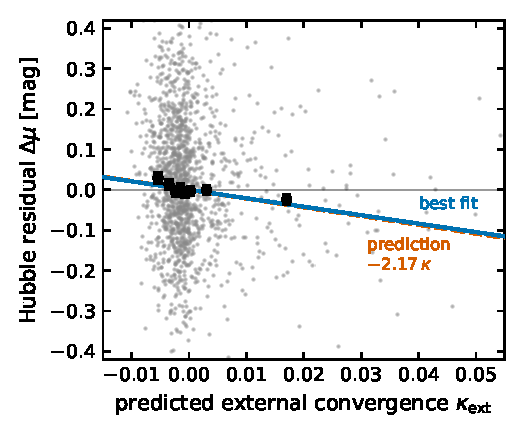
\includegraphics[width=\columnwidth]{fig1_slope.pdf}
\caption{Hubble residuals of 1450 DES-SN5YR SNe~Ia ($P_{\rm Ia}>0.9$;
gray points) against the predicted external convergence. Black points are
inverse-variance-weighted means in quantile bins of $\kext$. The best-fit
slope (blue) is $-2.10\pm0.47$; the a priori weak-lensing prediction
$-2.171\,\kext$ (vermilion dashed) is not a fit.
\label{fig:slope}}
\end{figure}

\section{Results}\label{sec:results}

Figure~\ref{fig:slope} shows the Hubble residuals against the predicted
convergence. A weighted linear fit gives
\begin{equation}
\frac{d\dmu}{d\kext} = -2.10 \pm 0.47~{\rm mag}
\qquad (N = 1450,\ P_{\rm Ia} > 0.9),
\end{equation}
with the uncertainty from bootstrap resampling; the full sample without
the probability cut gives $-2.09 \pm 0.47$. The ratio of observed to
predicted amplitude is
\begin{equation}
A \equiv \frac{b_{\rm fit}}{-5/\ln 10} = 0.96 \pm 0.22,
\end{equation}
a $4.4\sigma$ rejection of the no-lensing hypothesis with an amplitude
consistent with unity at the 4\% level. A Spearman rank test on the
unbinned pairs gives $\rho = -0.10$ with $p = 1\times10^{-4}$,
confirming the correlation non-parametrically. Splitting at
$\kext = 0.005$, the 202 high-convergence sight lines are brighter than
the remainder by $0.033 \pm 0.012$~mag ($2.8\sigma$), the direct
signature of magnification.

\begin{figure}
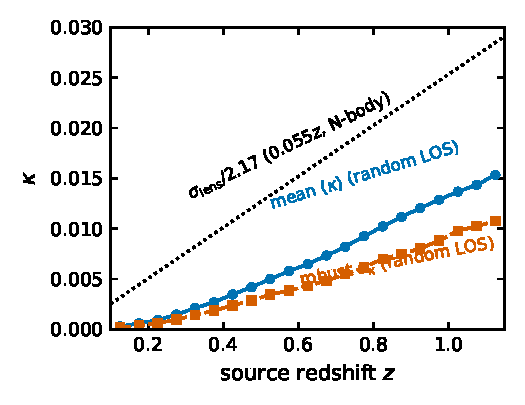
\includegraphics[width=\columnwidth]{fig2_zeropoint.pdf}
\caption{Redshift scaling of the random--sight-line convergence: the
mean (blue; the mass-sheet zero point) and robust scatter (vermilion) of
the catalog-halo convergence, compared with the total lensing scatter
from N-body expectations \citep[$0.055z$~mag, shown in convergence
units;][]{Jonsson2010}. Catalog halos account for $\sim$40--50\% of the
expected total dispersion; the remainder is diffuse large-scale structure
inaccessible to any galaxy-catalog method.
\label{fig:zp}}
\end{figure}

Figure~\ref{fig:zp} shows that both the zero point and the scatter of the
random--sight-line convergence grow with source redshift as expected,
with the catalog-halo scatter reaching $\sigma_\kappa \simeq 0.009$
($\simeq 0.020$~mag) at $z = 1$ --- roughly 40--50\% of the total N-body
lensing dispersion, quantifying the fraction of the lensing variance that
per--sight-line de-lensing can address in principle.

\begin{figure}
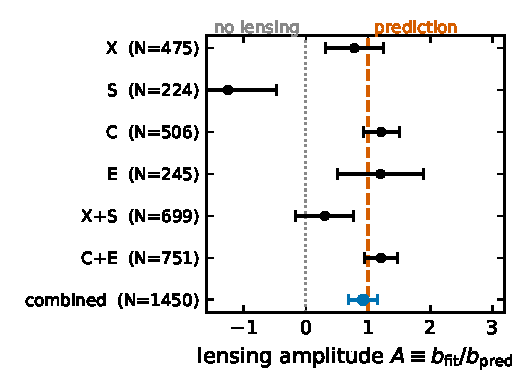
\includegraphics[width=\columnwidth]{fig3_forest.pdf}
\caption{Lensing amplitude by field group. All groups except Stripe~82
(S; $N=224$, the shallowest subsample) are consistent with the predicted
amplitude $A=1$; a jackknife over field groups keeps the combined slope
within $[-2.45, -1.55]$. \label{fig:forest}}
\end{figure}

\begin{deluxetable}{lcccc}
\tablecaption{Highest predicted-convergence sight lines
\label{tab:top}}
\tablehead{\colhead{CID} & \colhead{Field} & \colhead{$z_{\rm HD}$} &
\colhead{$\kext$} & \colhead{$\dmu$ [mag]}}
\startdata
1316989 & X1 & 0.553 & 0.123 & $-0.29$ \\
1260954 & E2 & 0.699 & 0.111 & $-0.05$ \\
1537077 & C3 & 0.745 & 0.099 & $-0.17$ \\
1337703 & C1 & 0.532 & 0.089 & $-0.34$ \\
1879483 & X3 & 0.876 & 0.087 & $-0.28$ \\
1880486 & S2 & 0.634 & 0.077 & $+0.32$ \\
1915087 & E2 & 0.561 & 0.073 & $-0.02$ \\
1339232 & C3 & 0.969 & 0.073 & $-0.25$ \\
1255169 & C3 & 1.047 & 0.072 & $-0.26$ \\
1450127 & X3 & 0.600 & 0.066 & $+0.03$ \\
\enddata
\tablecomments{Predicted magnifications of 0.14--0.27~mag; seven of ten
show negative (bright) Hubble residuals. These sight lines pass within
$\lesssim 1'$ of foreground clusters and merit individual attention in
cosmological analyses.}
\end{deluxetable}

Figure~\ref{fig:forest} and Table~\ref{tab:top} address robustness and
the tail. The amplitude is consistent across field groups except
Stripe~82, which prefers a positive slope at low weight ($N=224$;
$1.7\sigma$--$2\sigma$ from the other groups, consistent with a
statistical fluctuation); removing any single group leaves the detection
intact. Notably, the fields \emph{without} DESI spectroscopic coverage
(CDF-S, Elais-S1) carry the signal as strongly as the spectroscopy-rich
fields, indicating that at these source redshifts the convergence
fidelity is set by the depth of the photometric catalog and the cluster
model rather than by spectroscopic sharpening of the foreground kernel.
The highest-$\kext$ sight lines (Table~\ref{tab:top}) have predicted
magnifications of 0.14--0.27~mag, and seven of ten are indeed bright.

\section{Discussion}\label{sec:disc}

\emph{A population-level test of the galaxy--halo connection.} Because
the amplitude is predicted, $A = 0.96 \pm 0.22$ is a measurement: the
mean halo surface density implied by the adopted stellar-mass--halo-mass
relation, concentration model, truncation, and cluster masses reproduces
the lensing of 1450 standard candles to within 22\%. Given the
$\sim$0.7--0.8 logarithmic sensitivity of $\kappa$ to halo mass in this
regime, this bounds the effective halo-mass normalization of the model at
the $\sim$30\% level --- an SN-magnification analog of galaxy--galaxy
lensing calibrations, with entirely independent sources and systematics.

\emph{Relation to \citet{Shah2024}.} The two measurements are
complementary rather than competing. Shah et al. optimize a fitted
normalization and achieve $6.0\sigma$; we fix the normalization a priori
and achieve $4.4\sigma$ with the amplitude itself becoming the science
product. The agreement of their fitted mass-to-light ratios with
expectations and our $A \simeq 1$ are consistent statements from opposite
directions.

\emph{De-lensing and tail control.} The correctable dispersion,
$|b|\,\sigma_{\kext} \simeq 0.02$~mag at $z \sim 0.8$, remains a small
correction to the $\sim$0.2~mag total residual scatter, so
per--sight-line de-lensing will not materially tighten current
constraints --- consistent with \citet{Shah2024}. The operational value
lies in the tail: the released per-SN $\kext$ catalog converts the
skewness noted by \citet{Abbott2024} from an unmodeled nuisance into a
per-object flag, exonerating or implicating lensing for individual
Hubble-diagram outliers (Table~\ref{tab:top}) at the cost of a catalog
lookup. For deeper samples (LSST, {\it Roman}), where
$\sigma_{\rm lens}$ approaches the intrinsic scatter for the $z \gtrsim
1.5$ tail, both the de-lensing term and the amplitude test sharpen
substantially, and the present method --- 26 minutes for 1572 sight
lines from public catalogs --- scales trivially.

\emph{Caveats.} The prediction captures the one-halo term of catalog
objects relative to the field mean; diffuse structure contributes
additional, uncorrelated dispersion but should not bias the slope. Halo
masses derive from photometric estimators with 0.16~dex validated
scatter; cluster masses are richness-based with marginalized scatter and
miscentering. Host coordinates proxy the sight lines. None of these
enters the Hubble residuals, preserving the blind character of the
amplitude test.

\section{Summary}

Using only public catalogs and an independently calibrated halo model, we
predict the external convergence toward 1450 DES-SN5YR SNe~Ia and detect
the corresponding magnification at $4.4\sigma$, with an observed-to-predicted
amplitude of $0.96 \pm 0.22$. This is, to our knowledge, the first
supernova lensing detection in which the amplitude is a genuine
prediction, turning lensed standard candles into a test of the
galaxy--halo connection and providing a per-object magnification catalog
for the DES five-year cosmological sample.

\begin{acknowledgments}
This work used the public DES-SN5YR data release, data products of the
DESI Legacy Imaging Surveys (DR10) and DESI DR1, the \citet{WenHan2024}
cluster catalog via CDS/VizieR, and services provided by the Astro Data
Lab, part of the Community Science and Data Center Program of NSF
NOIRLab. P.E.N. acknowledges support from the DOE Office of Science,
Office of High Energy Physics, under contract DE-AC02-05CH11231.
Anthropic's Claude was used to assist in the analysis and the drafting
of this manuscript.
\end{acknowledgments}

\facilities{Blanco (DECam), Mayall (DESI, Mosaic-3), Bok (90Prime), WISE}
\software{\snk\ (\url{https://github.com/nugent68/SNKappa}), astropy,
numpy, scipy, colossus \citep{Diemer2018}, pyvo}

\section*{Data Availability}
The per-supernova $\kext$ catalog, the analysis scripts, and the full
query provenance are available at
\url{https://github.com/nugent68/SNKappa} (\texttt{scripts/des\_full.py};
\texttt{output/des\_full/des\_all\_kappa.csv}).

\begin{thebibliography}{}
\bibitem[Abbott et al.(2024)]{Abbott2024} Abbott, T.~M.~C., Acevedo, M.,
Aguena, M., et al. 2024, ApJL, 973, L14
\bibitem[Baltz et al.(2009)]{BMO2009} Baltz, E.~A., Marshall, P., \&
Oguri, M. 2009, JCAP, 2009, 015
\bibitem[Behroozi et al.(2013)]{Behroozi2013} Behroozi, P.~S., Wechsler,
R.~H., \& Conroy, C. 2013, ApJ, 770, 57
\bibitem[Ben\'itez et al.(2002)]{Benitez2002} Ben\'itez, N., Riess, A.,
Nugent, P., et al. 2002, ApJ, 577, L1
\bibitem[DESI Collaboration et al.(2025)]{DESI2025} DESI Collaboration,
Abdul-Karim, M., Adame, A.~G., et al. 2025, arXiv:2503.14745
\bibitem[Dey et al.(2019)]{Dey2019} Dey, A., Schlegel, D.~J., Lang, D.,
et al. 2019, AJ, 157, 168
\bibitem[Diemer(2018)]{Diemer2018} Diemer, B. 2018, ApJS, 239, 35
\bibitem[Diemer \& Joyce(2019)]{DiemerJoyce2019} Diemer, B., \& Joyce,
M. 2019, ApJ, 871, 168
\bibitem[Goobar et al.(2026)]{Goobar2026} Goobar, A., Johansson, J.,
M\"ortsell, E., et al. 2026, ApJ, in press
\bibitem[Holz \& Linder(2005)]{Holz2005} Holz, D.~E., \& Linder, E.~V.
2005, ApJ, 631, 678
\bibitem[J\"onsson et al.(2010)]{Jonsson2010} J\"onsson, J., Sullivan,
M., Hook, I., et al. 2010, MNRAS, 405, 535
\bibitem[Kettlety et al.(2018)]{Kettlety2018} Kettlety, T., Hesling, J.,
Phillipps, S., et al. 2018, MNRAS, 473, 776
\bibitem[Meidt et al.(2014)]{Meidt2014} Meidt, S.~E., Schinnerer, E.,
van de Ven, G., et al. 2014, ApJ, 788, 144
\bibitem[Nugent et al.(2025)]{Nugent2025} Nugent, A.~E., Villar,
V.~A., Gagliano, A., et al. 2025, ApJ, in press (arXiv:2509.08874)
\bibitem[S\'anchez et al.(2024)]{Sanchez2024} S\'anchez, B.~O., Brout,
D., Vincenzi, M., et al. 2024, ApJ, 975, 5
\bibitem[Shah et al.(2022)]{Shah2022} Shah, P., Lemos, P., \& Lahav, O.
2022, MNRAS, 515, 2305
\bibitem[Shah et al.(2024)]{Shah2024} Shah, P., Davis, T.~M., Bacon,
D., et al. 2024, MNRAS (arXiv:2406.05047)
\bibitem[Vincenzi et al.(2024)]{Vincenzi2024} Vincenzi, M., Brout, D.,
Armstrong, P., et al. 2024, ApJ, 975, 86
\bibitem[Wen \& Han(2024)]{WenHan2024} Wen, Z.~L., \& Han, J.~L. 2024,
ApJS, 272, 39
\bibitem[Zhou et al.(2021)]{Zhou2021} Zhou, R., Newman, J.~A., Mao,
Y.-Y., et al. 2021, MNRAS, 501, 3309
\end{thebibliography}

\end{document}
